\subsection{Chapter 11 - Rotational energy and momentum}

\subsubsection{Overview}\label{chapter:angularmomentumrolling}

In this chapter, we extend our description of rotational dynamics to include the rotational equivalents of kinetic energy and momentum. We also develop the framework for describing the motion of rolling objects. We will see that many of the relations that hold for linear quantities also hold for angular quantities.

\begin{framed}
\textbf{Learning Objectives}\\
\begin{itemize}
\item Understand how to define the rotational kinetic energy of an object as well as its total kinetic energy.
\item Understand how to model rolling motion, and what slipping means in the context of rolling motion.
\item Understand how to define the angular momentum of an object and when it is conserved.
\end{itemize}

\begin{framed}
\textbf{Think About It}\\
How can you model the motion of a downwards going yo-yo?

\begin{enumerate}
\item It is similar to that of an object falling with a force of drag.
\item It is similar to that of an object rolling down an incline.
\item It is similar to that of an object sliding down an incline.
\item It is similar to that of an object rotating about a fixed axis of rotation.
\end{enumerate}

\begin{framed}
\textbf{Answer}\\
\begin{enumerate}[resume]
\item
\end{enumerate}
\end{framed}
\end{framed}
\end{framed}

\subsubsection{Rotational kinetic energy of an object}

In this section, we show how to define the rotational kinetic energy of an object that is rotating about a stationary axis in an inertial frame of reference. Consider a solid object that is rotating about an axis with angular velocity, $\vec\omega$, as depicted in Figure~\ref{fig:angularmomentumrolling:rotE}.

\begin{figure}[!htbp]
\centering
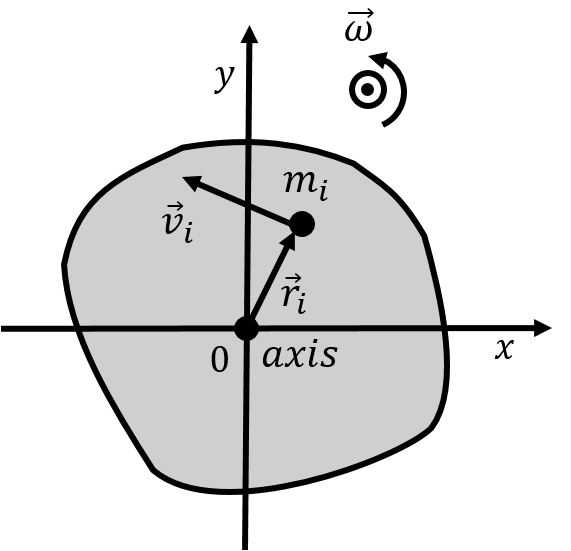
\includegraphics[width=0.4\linewidth]{files/rotE-3c26b1af2248a765fa579be7b104af95.png}
\caption[]{An object rotating about an axis that is perpendicular to the page.}
\label{fig:angularmomentumrolling:rotE}
\end{figure}

We can model the object as being composed of many point particles, each with a mass $m_i$, located at a position $\vec r_i$, with velocity $\vec v_i$ relative to the axis of rotation. We choose a coordinate system whose origin is on the axis of rotation and whose $z$ axis is co-linear with the axis of rotation, as depicted in Figure~\ref{fig:angularmomentumrolling:rotE}.

Each particle of mass $m_i$ in the object has a kinetic energy, $K_i$:
\begin{equation}
K_i = \frac{1}{2}m_iv_i^2
\end{equation}
We can sum the kinetic energy of each particle together to get the total rotational kinetic energy, $K_{rot}$, of the object:
\begin{equation}
K_{rot} = \sum_i \frac{1}{2}m_iv_i^2
\end{equation}
Although each particle will have a different velocity, $\vec v_i$, they will all have the same angular velocity, $\vec\omega$. For any particle, located a distance $r_i$ from the axis of rotation, their velocity is related to the angular velocity of the object by:
\begin{equation}
\vec v_i &= \vec \omega \times \vec r_i\\
v_i &= \omega r_i
\end{equation}
where $\vec \omega$ and $\vec r_i$ are always perpendicular to each other, since $\vec\omega$ is out of the plane of the page. Furthermore, the velocity vector, $\vec v_i$, will always be perpendicular to $\vec r_i$, since all particles are moving in circles centred about the axis of rotation.  We can thus write the total rotational kinetic energy of the object using the angular speed:
\begin{equation}
K_{rot} &= \sum_i \frac{1}{2}m_iv_i^2 = \sum_i \frac{1}{2}m_ir_i^2\omega^2= \frac{1}{2} \omega^2 \sum_i m_ir_i^2\\
&=\frac{1}{2}I\omega^2
\end{equation}
where we factored $\omega$ and the one half out of the sum, as these are the same for each particle $i$. We then recognized that the remaining sum is simply the definition of the object's moment of inertia about the axis:
\begin{equation}
I = \sum_i mr_i^2
\end{equation}

Thus, the rotational kinetic energy of an object rotating with angular speed $\omega$ about an axis that is stationary in an inertial frame of reference is given by:
\begin{equation}
\boxed{K_{rot}=\frac{1}{2}I\omega^2}
\end{equation}
where $I$ is the object's moment of inertia about that axis. The rotational kinetic energy is functionally very similar to the linear kinetic energy; instead of mass, we use the moment of inertia, and instead of speed squared, we use angular speed squared.

\paragraph{Work on a rotating object}

We can calculate the work done by a force exerted on an object rotating about a stationary axis in an inertial frame of reference. Let $\vec F$ be a force exerted at position, $\vec r$, relative to the axis of rotation at some instant in time, and let the force be exerted in the plane perpendicular to the axis of rotation, as illustrated in Figure~\ref{fig:angularmomentumrolling:work}. Because the object is rotating about the given axis, only the component of the force that is tangent to the circle about which the point where the force is exerted can do work (only the component of the force that is parallel to the displacement can do work).

The work done by the force as the object rotates by a certain angle is given by:
\begin{equation}
W = \int \vec F \cdot d\vec l = \int F_\perp dl
\end{equation}
where $d\vec l$ is a small displacement along the (circular) path followed by the point where the force is exerted, as illustrated in Figure~\ref{fig:angularmomentumrolling:work}. $F_\perp$ is the component of $\vec F$ that is perpendicular to the vector, $\vec r$, from the axis of rotation to the location where the force is exerted ($F_\perp$ is the component of $\vec F$ that is tangent to the circle).

\begin{figure}[!htbp]
\centering
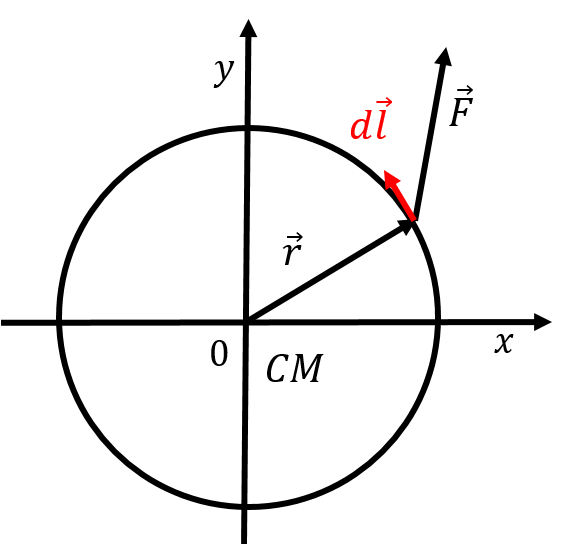
\includegraphics[width=0.4\linewidth]{files/work-84fbe3453bb9868e829beb7d99b979d9.png}
\caption[]{Calculating the work done by a force on a rotating object.}
\label{fig:angularmomentumrolling:work}
\end{figure}

At some instant in time, when the force is exerted at position, $\vec r$, consider the scalar product between the torque from the force, $\vec \tau$, and an infinitesimal angular displacement, $d\vec \theta$, about the axis of rotation:
\begin{equation}
\vec\tau \cdot d\vec\theta = (\vec r \times \vec F) \cdot \left(\frac{1}{r^2} \vec r\times d\vec l\right)
\end{equation}
The vectors $\vec \tau$ and $d\vec \theta$ are parallel to the axis of rotation (because $\vec F$ and $d\vec l$ are in the plane perpendicular to the axis of rotation), so their scalar product will be equal to the product of their magnitudes. The vector $\vec r \times \vec F$ has a magnitude of:
\begin{equation}
\vec r \times \vec F = rF_\perp
\end{equation}
where $F_\perp$ is the component of the force tangent to the circle. The vector $\vec r\times d\vec l$ has a magnitude:
\begin{equation}
\vec r\times d\vec l = rdl
\end{equation}
since $\vec r$ and $d\vec l$ are always perpendicular. The scalar product $\vec\tau \cdot d\vec\theta$ is thus equal to:
\begin{equation}
\vec\tau \cdot d\vec\theta = rF_\perp \frac{1}{r^2} rdl = F_\perp dl
\end{equation}
The work done by a force when an object rotates about an axis can thus be written in terms of its torque about that axis and the corresponding angular displacement from $\theta_1$ to $\theta_2$:
\begin{equation}
W = \int_{\theta_1}^{\theta_2}\vec\tau\cdot d\vec \theta
\end{equation}

The net work done on an object through an angular displacement from $\theta_1$ to $\theta_2$ can thus be written using the net torque $\vec \tau^{net}$ exerted on the object:
\begin{equation}
W^{net} = \int_{\theta_1}^{\theta_2}\vec\tau^{net}\cdot d\vec \theta
\end{equation}
We can re-arrange this using Newton's Second Law for rotational dynamics:
\begin{equation}
\vec\tau^{net} &= I \vec\alpha\\
&= I \frac{d\vec\omega}{dt} =  I \frac{d\omega}{d\theta}\frac{d\vec\theta}{dt}=I \frac{d\omega}{d\theta} \vec\omega
\end{equation}
which allows us to write the integral over a change in angular velocity instead of angular displacement:
\begin{equation}
W^{net} &= \int_{\theta_1}^{\theta_2}\vec\tau^{net}\cdot d\vec \theta =  \int_{\theta_1}^{\theta_2}I \frac{d\omega}{d\theta} \vec\omega \cdot d\vec \theta\\
&=\int_{\omega_1}^{\omega_2}I \omega d\omega = \frac{1}{2}I\omega_2^2 - \frac{1}{2}I\omega_1^2
\end{equation}
where we used the fact that $\vec\omega$ are $d\vec\theta$ are parallel. We thus find that the Work-Energy Theorem can also be applied to find the change in rotational kinetic energy resulting from the net work done by a torque:
\begin{equation}
\boxed{W^{net}=\int_{\theta_1}^{\theta_2}\vec\tau^{net}\cdot d\vec \theta = \Delta K_{rot}}
\end{equation}

If a constant torque, $\vec\tau$, is exerted on an object that is rotating at constant angular velocity, $\vec\omega$, then the rate at which that work  is being done is given by:
\begin{equation}
P = \frac{dW}{dt} = \frac{d}{dt} \vec \tau \cdot d\vec\theta =  \vec \tau \cdot \frac{d\vec\theta}{dt} = \vec \tau \cdot \vec\omega
\end{equation}
This is very similar to the power, $P=\vec F\cdot \vec v$, with which a force does work on an object moving with constant velocity, except that instead of force we use torque, and instead of velocity, we use angular velocity.

\paragraph{Total kinetic energy of an object}

In the frame of reference of the centre of mass, an object rotating about an axis through its centre of mass with angular velocity, $\vec \omega$, will have rotational kinetic energy, $K_{rot}$, given by:
\begin{equation}
K_{rot}=\frac{1}{2}I_{CM}\omega^2
\end{equation}
where $I_{CM}$ is the moment of inertia of the object about the axis through its centre of mass.

We wish to determine the kinetic energy of the object in an inertial frame of reference where the object's centre of mass is moving with a velocity $\vec v_{cm}$; that is, in a frame where the axis of rotation is moving with the velocity of the centre of mass. We model the object as being composed of particles of mass, $m_i$, each located at position, $\vec r_i$, relative to the axis of rotation through the centre of mass. The velocity, $\vec v_i$, of a particle $i$, in this frame of reference, is given by:
\begin{equation}
\vec v_i = \vec\omega \times \vec r_i + \vec v_{CM}
\end{equation}
where $\vec\omega \times \vec r_i$ is the velocity of the particle as seen in the centre of mass (due to rotation). The kinetic energy of particle $i$, $K_i$, is given by:
\begin{equation}
K_i = \frac{1}{2}m_iv_i^2 = \frac{1}{2}m_i(\vec v_i\cdot \vec v_i)
\end{equation}
where we expressed the speed of the particle squared using a scalar product of the velocity of the particle with itself. The total kinetic energy of the object is found by summing the kinetic energies of all of the particles:
\begin{equation}
K_{tot} &= \sum \frac{1}{2}m_i(\vec v_i\cdot \vec v_i) \\
&=\frac{1}{2} \sum_i m_i (\vec\omega \times \vec r_i + \vec v_{CM}) \cdot (\vec\omega \times \vec r_i + \vec v_{CM})\\
&=\frac{1}{2} \sum_i m_i (\vec\omega \times \vec r_i)\cdot(\vec\omega \times \vec r_i ) + \frac{1}{2} \sum_i m_i (\vec v_{CM}) \cdot (\vec v_{CM}) + \sum_i m_i (\vec\omega \times \vec r_i) \cdot (\vec v_{CM})\\
&=\frac{1}{2}  \sum_i m_i \omega^2r_i^2 + \frac{1}{2} \sum_i m_i v_{CM}^2 + \sum_i m_i (\vec\omega \times \vec r_i) \cdot (\vec v_{CM})\\
&=\frac{1}{2} I_{CM}\omega ^2 + \frac{1}{2}M v_{CM}^2+\sum_i m_i (\vec\omega \times \vec r_i) \cdot (\vec v_{CM})
\end{equation}
where the first term is the rotational kinetic energy that we found earlier. The second term, called the ``translational kinetic energy'', can be thought of as the kinetic energy of the whole system with mass $M=\sum m_i$, due to the translational motion of the centre of mass. The last term is identically zero; we can re-order the scalar product and factor $\vec v_{CM}$ out of the sum:
\begin{equation}
\sum_i m_i (\vec\omega \times \vec r_i) \cdot (\vec v_{CM}) &= (\vec v_{CM}) \cdot \sum_i m_i (\vec\omega \times \vec r_i)\\
&=(\vec v_{CM}) \cdot \sum_i m_i \vec v'_{i}
\end{equation}
where $v'_{i} = \vec\omega \times \vec r_i$ is the velocity of particle $i$ in the center of mass frame of reference. But the sum:
\begin{equation}
\sum_i m_i \vec v'_{i}
\end{equation}
is the numerator for the definition of the velocity of the centre of mass, which, in the centre of mass frame of reference is identically zero!

Thus, the total kinetic energy of an object of mass, $M$, that is rotating about an axis through its centre of mass with angular velocity, $\omega$, and whose centre of mass is moving with velocity, $\vec v_{CM}$, is given by:
\begin{equation}
\boxed{K_{tot}=K_{rot}+K_{trans}=\frac{1}{2} I_{CM}\omega ^2 + \frac{1}{2}M v_{CM}^2}
\end{equation}
The total kinetic energy can be thought of as the sum of the rotational and kinetic energies.

\subsubsection{Rolling motion}

In this section, we examine how to model the motion of an object that is rolling along a surface, such as the motion of a bicycle wheel. Consider the motion of a wheel of radius, $R$, rotating with angular velocity, $\vec\omega$, about an axis perpendicular to the wheel and through its centre of mass, \textbf{as observed in the centre of mass frame}. This is illustrated in Figure~\ref{fig:angularmomentumrolling:wheelcm}.

\begin{figure}[!htbp]
\centering
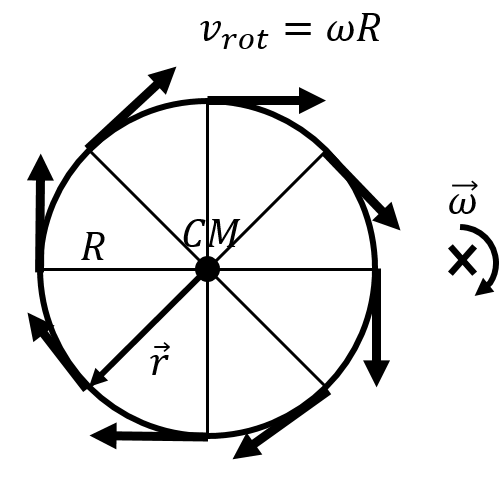
\includegraphics[width=0.3\linewidth]{files/wheelcm-0e33844708b1777dab52fec6eb370889.png}
\caption[]{A wheel rotating with angular velocity $\vec\omega$ about an axis through its centre of mass.}
\label{fig:angularmomentumrolling:wheelcm}
\end{figure}

In the frame of reference of the centre of mass, each point on the edge of the wheel has a velocity, $\vec v_{rot}$, due to rotation given by:
\begin{equation}
\vec v_{rot} = \vec \omega\times \vec r
\end{equation}
where $\vec r$ is a vector (of magnitude $R$) from the centre of mass to the corresponding point on the edge of the wheel (shown in Figure~\ref{fig:angularmomentumrolling:wheelcm} for a point on the lower left of the wheel). The vector $\vec r$ is always perpendicular to $\vec \omega$, so that the speed of all points on the edge, as measured in the frame of reference of the centre of mass, is the same:
\begin{equation}
\label{eq:angularmomentumrolling:vrot}
v_{rot} = \omega R
\end{equation}
as illustrated in Figure~\ref{fig:angularmomentumrolling:wheelcm}.

Now, suppose that the whole wheel is moving, as it rolls on the ground, such that the centre of mass of the wheel moves with a velocity, $\vec v_{CM}$, as illustrated in Figure~\ref{fig:angularmomentumrolling:wheelground}.

\begin{figure}[!htbp]
\centering
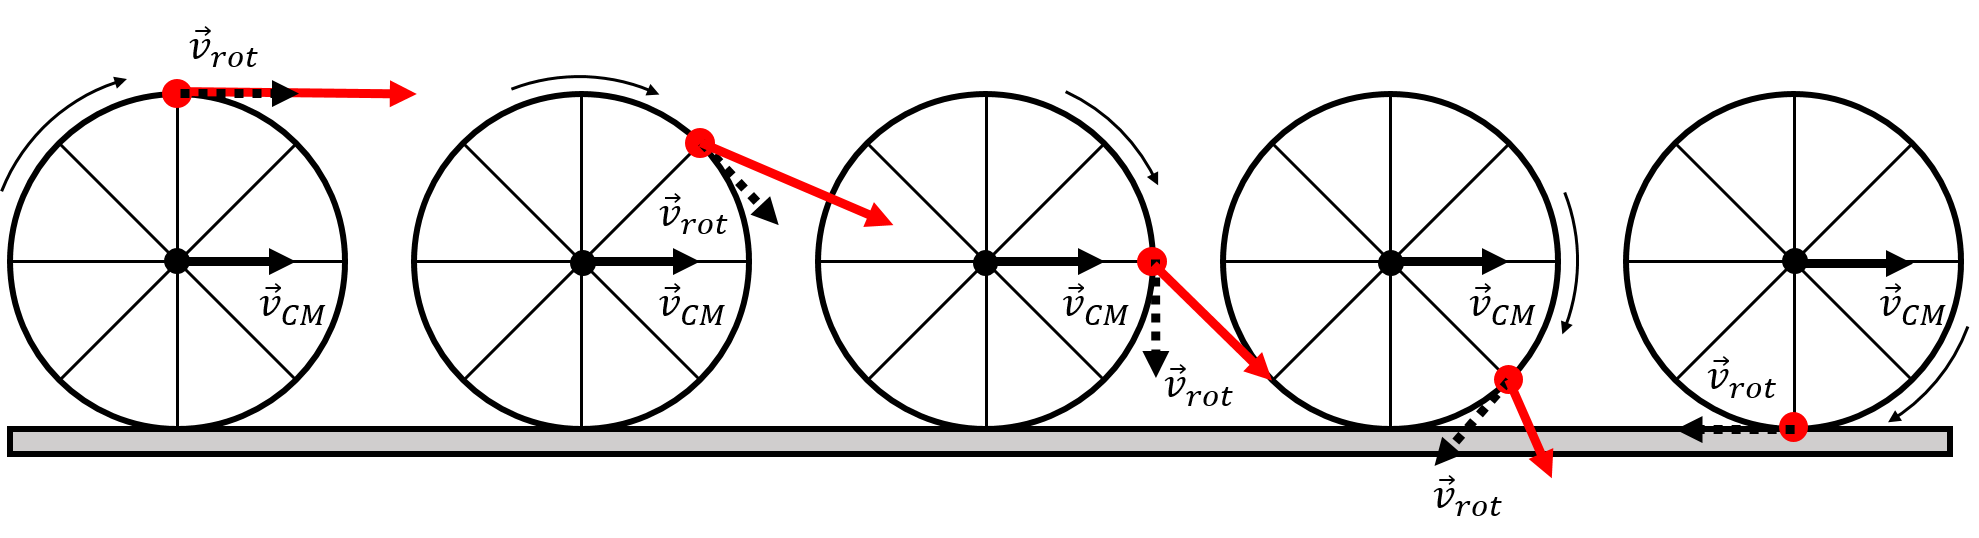
\includegraphics[width=0.95\linewidth]{files/wheelground-ea054c3bfbed539816b3e6d137584dbb.png}
\caption[]{A wheel rolling without slipping on the ground, with the centre of mass moving with velocity $\vec v_{CM}$.}
\label{fig:angularmomentumrolling:wheelground}
\end{figure}

The wheel is shown at different instants in time, as the point shown in red moves around the centre of mass.\}
In the frame of reference of the ground, each point on the edge of the wheel will have a velocity $\vec v$ given by:
\begin{equation}
\vec v = \vec v_{rot} + \vec v_{CM}
\end{equation}
That is, in the frame reference of the ground, each point will have a velocity obtained by (vectorially) adding its velocity relative to the centre of mass, $\vec v_{rot}$, and the velocity of the centre of mass relative to the ground, $\vec v_{CM}$. This is illustrated in Figure~\ref{fig:angularmomentumrolling:wheelground} for one specific point, shown in red. The red vector corresponds to the velocity of the red point as the wheel rotates, and is obtained by adding the velocity of the centre of mass, $\vec v_{CM}$, and the velocity, $\vec v_{rot}$, relative to the centre of mass (shown as the dashed vector, tangent to the edge of the wheel).

Consider, specifically, the instant in time when the red point is at the bottom of the wheel, where the wheel makes contact with the ground. \textbf{If the wheel is not slipping with respect to the ground}, then the point is, at that instant, at rest relative to the ground. We call this type of motion ``rolling without slipping''; the point on the rotating object that is in contact with the ground is instantaneously at rest relative to the ground. This is the scenario illustrated in Figure~\ref{fig:angularmomentumrolling:wheelground}.

For the point in contact with the ground, the vectors $\vec v_{rot}$ and $\vec v_{CM}$ are anti-parallel, horizontal, and must sum to zero. Writing out the horizontal component of the velocity of that point (choosing the positive direction to be in the direction of the velocity of the centre of mass):
\begin{equation}
v &= -v_{rot} + v_{CM} = 0\\
\therefore v_{rot} &= v_{CM}
\end{equation}
and we find that, for rolling without slipping, the speed due to rotation about the centre of mass has to be equal to the speed of the centre of mass. The speed due to rotation about the centre of mass can be expressed using the angular velocity of the wheel about the centre of mass ((\ref{eq:angularmomentumrolling:vrot})). For rolling without slipping, we thus have the following relationship between angular velocity and the speed of the centre of mass:
\begin{equation}
\boxed{\omega R = v_{CM}}\quad \text{(rolling without slipping)}
\end{equation}
It makes sense for the angular velocity to be related to the speed of the centre of mass. The faster the wheel rotates, the faster the centre of mass will move. If the wheel is slipping with respect to the ground, then the point of contact is no longer stationary relative to the ground, and there is no relation between the angular velocity and the speed of the centre of mass. For rolling with slipping, imagine the motion of your bicycle wheel as you try to ride your bike on a slick sheet of ice.

For rolling without slipping, the magnitude of the linear acceleration of the centre of mass, $a_{CM}$, is similarly related to the magnitude of the angular acceleration of the wheel, $\alpha$, about the centre of mass:
\begin{equation}
a_{CM} &= \frac{dv_{CM}}{dt} = \frac{d}{dt}\omega R = R \frac{d\omega}{dt}\\
\therefore a_{CM} &= R\alpha
\end{equation}

\begin{framed}
\textbf{Checkpoint}\\
For rolling without slipping (Figure~\ref{fig:angularmomentumrolling:wheelground}), the speed of the point on the wheel that is in contact with the ground is 0. What is the speed of the point at the top of the wheel?

\begin{enumerate}
\item 0
\item $v_{CM}$.
\item $2v_{CM}$.
\item None of the above.
\end{enumerate}

\begin{framed}
\textbf{Answer}\\
\begin{enumerate}[resume]
\item
\end{enumerate}
\end{framed}
\end{framed}

\begin{framed}
\textbf{Example 11.1}\\
\begin{figure}[!htbp]
\centering
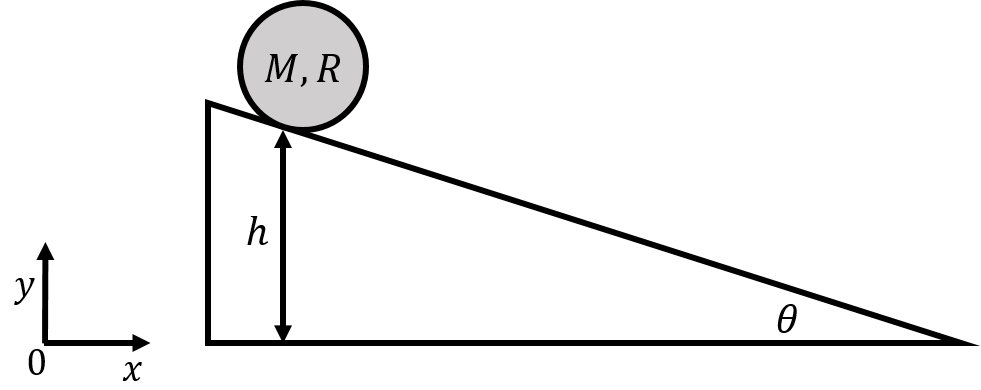
\includegraphics[width=0.5\linewidth]{files/diskslope-7e1ab66d6b3e0fd4d814dc76ee898212.png}
\caption[]{A disk rolling without slipping down an incline.}
\label{fig:angularmomentumrolling:diskslope}
\end{figure}

A disk of mass $M$ and radius $R$ is placed on an incline at a height $h$ above the ground. The incline makes an angle $\theta$ with respect to the horizontal, as shown in Figure~\ref{fig:angularmomentumrolling:diskslope}. If the disk starts at rest and rolls without slipping down the incline, what speed will the centre of mass have when the disk reaches the bottom of the incline?

\begin{framed}
\textbf{Solution}\\
We can use the conservation of mechanical energy to determine the speed of the centre of mass at the bottom of the incline, as there are no non-conservative forces doing work on the disk. If we choose to define gravitational potential energy such that it is zero at the bottom of the incline, we can write the total mechanical energy of the disk at the top of the incline as:
\begin{equation}
E = K+U=(0)+Mgh
\end{equation}
where the kinetic energy is zero, since the disk starts at rest\footnote{Technically, the potential energy should be taken for the height of the centre of mass, which is a distance $h_{CM}=h+R\cos\theta$ from the ground at the top of the incline, and a height $h'_{CM}=R$ at the bottom of the incline. The net difference in height for the centre of mass is thus $h_{CM} -h'_{CM} = h+R(1 -\cos\theta)$. If we assume that $h$ is much bigger than $R$, then this is negligible, otherwise, that is what we should use instead of $h$ for the potential energy.}. At the bottom of the incline, the disk will have only kinetic energy, since the potential energy at the bottom is defined to be zero. The kinetic energy of the disk will have a component from the rotation of the disk about the centre of mass, with angular speed $\omega$, and a component from the translation of the centre of mass with speed $v_{CM}$. The mechanical energy at the bottom of the incline is thus:
\begin{equation}
E' = K' + U = K'_{rot}+K'_{trans}+(0)=\frac{1}{2}I_{CM}\omega^2 + \frac{1}{2}Mv_{cm}^2
\end{equation}
Since the disk is rolling without slipping, its angular speed is related to the speed of centre of mass:
\begin{equation}
\omega = \frac{v_{CM}}{R}
\end{equation}
The moment of inertia of the disk about its centre of mass is given by:
\begin{equation}
I_{CM}=\frac{1}{2}MR^2
\end{equation}
We can thus write the mechanical energy at the bottom of the incline as:
\begin{equation}
E' &= \frac{1}{2}I_{CM}\omega^2 + \frac{1}{2}Mv_{cm}^2\\
&=\frac{1}{2}\left(  \frac{1}{2}MR^2 \right) \left(  \frac{v_{CM}}{R}\right)^2+ \frac{1}{2}Mv_{cm}^2\\
&=\frac{3}{4}Mv_{cm}^2
\end{equation}
Applying conservation of energy allows us to determine the speed of the centre of mass at the bottom of the incline:
\begin{equation}
E &= E'\\
Mgh &= \frac{3}{4}Mv_{cm}^2\\
\therefore v_{CM} &= \sqrt{\frac{4}{3}gh}
\end{equation}

\textbf{Discussion:} This example showed how we can use the conservation of energy to model the motion of an object that is rolling without slipping. The constraint of rolling without slipping allowed for the angular speed of the object to be related to the speed of its centre of mass.
\end{framed}
\end{framed}

\begin{framed}
\textbf{Checkpoint}\\
A hoop, a disk, and a sphere roll without slipping down an incline. If they are all released at the same time, in what order will they arrive at the bottom?\}

\begin{enumerate}
\item Hoop, disk, sphere.
\item Sphere, disk, hoop.
\item Disk, sphere, hoop.
\item Disk, hoop, sphere.
\end{enumerate}

\begin{framed}
\textbf{Answer}\\
\begin{enumerate}[resume]
\item
\end{enumerate}
\end{framed}
\end{framed}

\paragraph{The instantaneous axis of rotation}

When an object is rolling without slipping, we can model its motion as the superposition of rotation about the centre of mass and translational motion of the centre of mass, as in the previous section. However, because the point of contact between the rolling object and the ground is stationary, we can also model the motion as if the object were instantaneously rotating with angular velocity, $\vec \omega$, about a stationary axis through the point of contact. That is, we can model the motion as rotation only, with no translation, if we choose an axis of rotation through the point of contact between the ground and the wheel.

We call the axis through the point of contact the ``instantaneous axis of rotation'', since, instantaneously, it appears as if the whole wheel is rotating about that point. This is illustrated in Figure~\ref{fig:angularmomentumrolling:wheelinstant}, which shows, in red, the velocity vector for each point on the edge of the wheel, relative to the instantaneous axis of rotation. Because the axis of rotation is fixed to the ground, the velocity of each point about that axis of rotation corresponds to the same velocity relative to the ground that is depicted in Figure~\ref{fig:angularmomentumrolling:wheelground}.

\begin{figure}[!htbp]
\centering
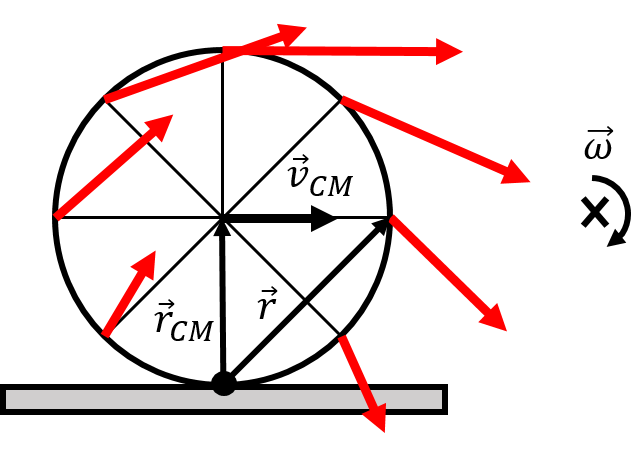
\includegraphics[width=0.4\linewidth]{files/wheelinstant-2a6ca6fe77408916b27c34e10ac10053.png}
\caption[]{A wheel that is rolling without slipping, as viewed if rotating about the instantaneous axis of rotation that passes through the point of contact with the ground.}
\label{fig:angularmomentumrolling:wheelinstant}
\end{figure}

In particular, the angular velocity, $\vec \omega$, about the instantaneous axis of rotation is the same as when we model the motion as translation plus rotation about the centre of mass ,as in the previous section. Indeed, relative to the instantaneous axis of rotation, the centre of mass must still have a velocity $\vec v_{CM}$, which is given by:
\begin{equation}
\vec v_{CM} &= \vec\omega \times \vec r_{CM}\\
\therefore v_{CM} &= \omega R
\end{equation}
where $\vec r_{CM}$ is the vector from the axis of rotation to the centre of mass. This is the same condition for rolling without slipping that we found before. Similarly, the velocity of any point on the wheel, relative to the ground, is given by:
\begin{equation}
\vec v = \vec\omega \times \vec r
\end{equation}
where $\vec r$ is the vector from the axis of rotation to the point of interest (shown in Figure~\ref{fig:angularmomentumrolling:wheelinstant} for the point on the right side of the wheel). In particular, the velocity vector (in red) for any point is always perpendicular to the vector $\vec r$ for that point, which was not necessarily obvious when modelling the motion as rotation plus translation, as in Figure~\ref{fig:angularmomentumrolling:wheelground}.

\begin{framed}
\textbf{Example 11.2}\\
\begin{figure}[!htbp]
\centering
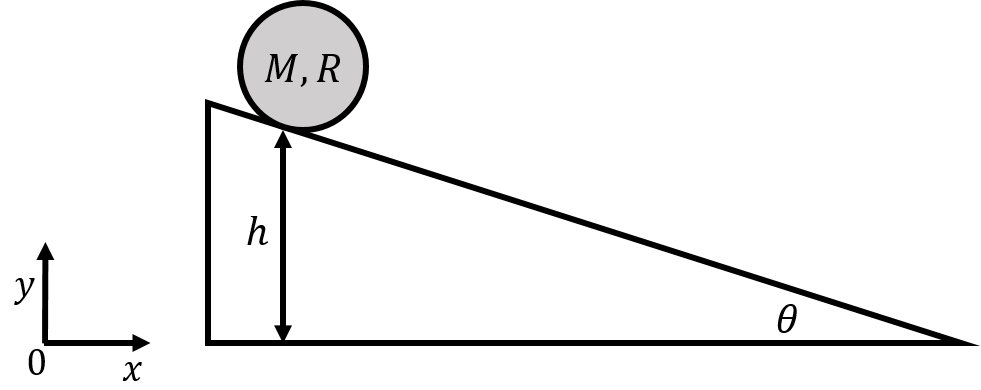
\includegraphics[width=0.5\linewidth]{files/diskslope-7e1ab66d6b3e0fd4d814dc76ee898212.png}
\caption[]{A disk rolling without slipping down an incline.}
\label{fig:angularmomentumrolling:diskslope2}
\end{figure}

A disk of mass $M$ and radius $R$ is placed on an incline at a height $h$ above the ground. The incline makes an angle $\theta$ with respect to the horizontal, as shown in Figure~\ref{fig:angularmomentumrolling:diskslope2}. What is the angular acceleration of the disk, about an axis through its centre of mass, as it rolls without slipping down the slope?

\begin{framed}
\textbf{Solution}\\
In order to determine the angular acceleration of the disk about the centre of mass, we need to model the forces that are exerted on the disk. The forces exerted on the disk are:

\begin{enumerate}
\item $\vec F_g$, the weight of the disk, exerted downwards at the centre of mass, with magnitude $Mg$.
\item $\vec N$, a normal force perpendicular to the incline, exerted by the incline at the point of contact with the disk.
\item $\vec f_s$, a force of static friction parallel to the incline, exerted by the incline at the point of contact with the disk. Without this force, the disk would simply slide down the incline without rotating.
\end{enumerate}

These forces are illustrated in Figure~\ref{fig:angularmomentumrolling:diskslope_fbd}, along with the acceleration of the centre of mass, and our choice of coordinate system (we choose the $x$ axis parallel to the acceleration of the centre of mass, to facilitate applying Newton's Second Law).

\begin{figure}[!htbp]
\centering
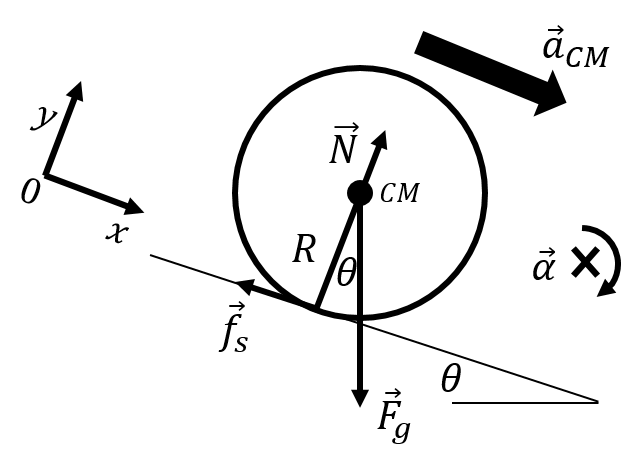
\includegraphics[width=0.4\linewidth]{files/diskslope_fbd-6c0bbf5637c869c1dcecbcc6a840deaf.png}
\caption[]{The forces on the disk rolling without slipping down an incline.}
\label{fig:angularmomentumrolling:diskslope_fbd}
\end{figure}

The angular acceleration of the disk about the centre of mass, $\vec \alpha$ is given by Newton's Second Law for rotational dynamics:
\begin{equation}
\vec\tau^{ext} = I_{CM}\vec\alpha
\end{equation}
where $\vec\tau^{ext}$ is the net external torque on the disk about the centre of mass (which will be in the negative $z$ direction).

The only force that can exert a torque about the centre of mass is the force of static friction. Gravity has a lever arm of zero and the normal force is anti-parallel to the vector that goes from the centre of mass to the point where the force is exerted. The net torque about the centre of mass is thus:
\begin{equation}
\vec\tau^{ext} = \vec \tau_{f_s} = \vec r_{f_s}\times \vec f_s= -Rf_s\hat z
\end{equation}
The angular acceleration will thus be in the negative $z$ direction, and the magnitude is given by:
\begin{equation}
\alpha = \frac{\tau^{ext}}{I_{CM}}=\frac{Rf_s}{\frac{1}{2}MR^2}=\frac{2f_s}{MR}
\end{equation}
However, we do not know the magnitude of the force of static friction. We can use the $x$ and $y$ components of Newton's Second Law to determine it (with acceleration of the centre of mass in the $x$ direction):
\begin{equation}
\sum F_x &= F_g\sin\theta - f_s = Ma_{CM}\\
\sum F_y &= N - F_g\cos\theta = 0
\end{equation}
Because the disk is rolling without slipping, the acceleration of the centre of mass is related to the angular acceleration of the disk:
\begin{equation}
a_{cm} = \alpha R
\end{equation}
The $x$ component of Newton's Second Law can thus be used to determine the magnitude of the force of static friction in terms of the angular acceleration:
\begin{equation}
Mg\sin\theta - f_s &= M \alpha R\\
\therefore f_s &= Mg\sin\theta - M\alpha R
\end{equation}
We can then substitute out the force of friction from our previous formula for the angular acceleration:
\begin{equation}
\alpha &= \frac{2f_s}{MR}\\
&=\frac{2Mg\sin\theta - 2M\alpha R}{MR} = \frac{2g\sin\theta}{R} - 2\alpha \\
\therefore \alpha &= \frac{2g\sin\theta}{3R}
\end{equation}

Instead of modelling the motion of the disk  as rotation about the centre of mass and translation of the center of mass, we can also model it about the instantaneous axis of rotation.

The angular acceleration about the instantaneous axis of rotation will be the same as the angular acceleration about the centre of mass. About the instantaneous axis of rotation, only the force of gravity can exert a torque, since the normal force and the force of friction both have a lever arm of zero. The torque from the force of gravity, about the instantaneous axis of rotation is:
\begin{equation}
\vec \tau_g = -F_gR\sin\theta \hat z = -MgR\sin\theta \hat z
\end{equation}
The torque from the force of gravity is equal to the moment of inertia of the disk about the instantaneous axis of rotation, $I$, multiplied by its angular acceleration:
\begin{equation}
\tau ^{ext} = \tau_g &= I\alpha\\
\therefore \alpha &= \frac{\tau_g}{I} = \frac{MgR\sin\theta}{I}
\end{equation}
The moment of inertia about the instantaneous axis of rotation is easily found using the parallel axis theorem:
\begin{equation}
I = I_{CM}+MR^2 = \frac{1}{2}MR^2 + MR^2 =\frac{3}{2}MR^2
\end{equation}
This allows us to find the angular acceleration of the disk:
\begin{equation}
\alpha &= \frac{MgR\sin\theta}{I} = \frac{MgR\sin\theta}{\frac{3}{2}MR^2}\\
&=\frac{2g\sin\theta}{3R}
\end{equation}
as we found previously, but in this case, we did not need to use Newton's Second Law to determine the force of friction.

\textbf{Discussion:} We saw that we can model the dynamics of the rolling body using either an axis through the centre of mass, or an axis through the instantaneous axis of rotation. The latter was easier in this case, because it did not require using Newton's Second Law.

By using an axis through the centre of mass to model the motion of the disk, it was clear that the force of static friction is required in order for the disk to rotate. Without the force of static friction, the disk would slide along the surface of the incline. The disk could still rotate if there is a force of kinetic friction that causes a torque that rotates the disk. If the surface were completely frictionless, the disk would simply slide down the incline, and we could model it as a sliding block. If the incline is too steep the force of static friction is no longer sufficient to provide the necessary torque required for the angular acceleration to be that which corresponds to rolling without slipping, and the disk would slip.
\end{framed}
\end{framed}

\subsubsection{Angular momentum}

In this section, we show that we can define a quantity called ``angular momentum'' as the rotational equivalent of the linear momentum.

\paragraph{Angular momentum of a particle}

The angular momentum relative to a point of rotation, $\vec L$, of a particle with linear momentum, $\vec p$, is defined as:
\begin{equation}
\boxed{\vec L = \vec r\times \vec p}
\end{equation}
where $\vec r$ is the vector from the point of rotation to the particle, and the linear momentum, $\vec p$, is defined relative to an inertial frame of reference in which the point of rotation is at rest.

Consider the time-derivative of angular momentum (where we have to use the product rule for derivatives):
\begin{equation}
\frac{d\vec L}{dt}  &= \frac{d}{dt} (\vec r\times \vec p)\\
&=\frac{d\vec r}{dt}\times \vec p + \vec r\times\frac{d\vec p}{dt}\\
&=\vec v\times \vec p + \vec r\times\frac{d\vec p}{dt}\\
\end{equation}
The first term is zero, since $\vec v$ is parallel to $\vec p$ by definition. Recall Newton's Second Law written using linear momentum:
\begin{equation}
\frac{d\vec p}{dt} = \vec F^{net}
\end{equation}
where $\vec F^{net}$ is the net force on the particle relative to the point of rotation. The rate of change of angular momentum is thus given by:
\begin{equation}
\frac{d\vec L }{dt} &= \vec r\times\frac{d\vec p}{dt}\\
&=\vec r\times\vec F^{net}
\end{equation}
where the term on the right is the net torque on the particle. Thus, the rate of change of angular momentum is given by:
\begin{equation}
\boxed{\frac{d\vec L}{dt}   = \vec \tau^{net}}
\end{equation}
which is analogous to the linear case, but we used angular momentum instead of linear momentum and net torque instead of net force. The net torque on a particle is thus equal to the rate of change of its angular momentum. In particular, the angular momentum of a particle will remain constant (not change with time) if the net torque on the particle is zero.

We can also define the angular momentum of a particle using only angular quantities:
\begin{equation}
\vec L = \vec r \times \vec p =  m \vec r \times \vec v = mr^2 \vec\omega
\end{equation}
where we factored the mass $m$ out of the momentum and used the definition $\vec \omega = 1/r^2(\vec r \times \vec v)$. We can think of $mr^2$ as the moment of inertia, $I$, of the particle and write:
\begin{equation}
\label{eq:angularmomentumrolling:liw}
\boxed{\vec L  = mr^2 \vec\omega = I \vec\omega}
\end{equation}
which is a close analogue to the definition of linear momentum, but we use moment of inertia instead of mass and angular velocity instead of velocity.

The angular momentum is thus parallel to the angular velocity of the particle about the point of rotation. If no net torque is exerted on the particle about that point, then the particle's angular momentum about that point will remain constant. We can also consider the torque and angular momentum about an axis instead of a point; in that case, we would simply take the components of torque and angular momentum that are parallel to that axis.

\begin{framed}
\textbf{Example 11.3}\\
\begin{figure}[!htbp]
\centering
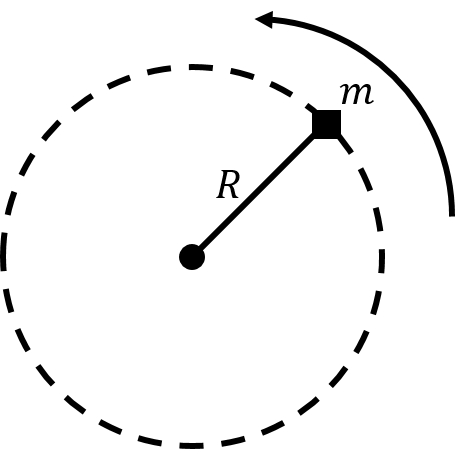
\includegraphics[width=0.25\linewidth]{files/circle-d31ab27f0e6119d03652d0284fcc0b14.png}
\caption[]{A small block attached to a mass-less string moving in a horizontal circle on a table.}
\label{fig:angularmomentumrolling:circle}
\end{figure}

A small block of mass $m$ attached to a mass-less string is moving along a circle of radius $R$ on a horizontal table, as depicted from above in Figure~\ref{fig:angularmomentumrolling:circle}. If the table is frictionless: are the block's linear and/or angular momentum with respect to the axis of rotation conserved? If there is friction between the table and the block, are the block's linear and/or angular momentum with respect to the axis of rotation conserved? What can you say about the kinetic energy of the block in the two cases?

\begin{framed}
\textbf{Solution}\\
If there is no friction between the block and the table, then the forces exerted on the block are:

\begin{enumerate}
\item $\vec F_g$, the block's weight, exerted downwards, with magnitude $mg$.
\item $\vec N$, a normal force, exerted upwards, with magnitude $mg$.
\item $\vec T$, a force of tension, exerted towards the centre of the circle.
\end{enumerate}

All of these forces are perpendicular to the (tangential) displacement of the block along the circle. Thus, there can be no work done on the block and its speed, $v$, must remain constant. The kinetic energy of the block must thus remain constant.

The sum of the forces on the block must be towards the centre of the circle, since the block is in uniform circular motion. The linear momentum of the block cannot be conserved if there is a net force on the block (and clearly, the block's velocity vector changes direction as it goes around the circle).

The forces of weight and the normal force are both outside of the plane of motion, and thus cannot exert a torque along the axis of rotation. They are also equal and opposite in magnitude so the net torque from those two forces is always zero (since the net force from those forces is zero). The force of tension is always anti-parallel to the vector $\vec r$, from the axis of rotation to the particle, and cannot result in a torque about the rotation axis. Thus, the net torque on the block is zero and its angular momentum must be conserved.

If there is kinetic friction exerted by the table on the block, then there is an additional force, $\vec f_s$, exerted on the block in the direction opposite of motion (tangent to the circle, in the opposite direction from the block's velocity).

The force of friction will do negative work on the block, slowing it down and reducing its kinetic energy, which is no longer conserved. The net force on the block is non-zero, so its linear momentum is still not conserved. Finally, the force of friction, which is always perpendicular to $\vec r$, will result in a torque that reduces the angular velocity of the block. The block's angular momentum is thus no longer conserved when there is friction between the table and the block.

\textbf{Discussion:} In this example, we saw that kinetic energy, linear momentum, and angular momentum are all conserved under different conditions. Kinetic energy is conserved if no net work is done on the block. Linear momentum is conserved if the net force on the block is zero. Angular momentum is conserved if the net torque on the block is zero. By introducing angular momentum, we are able to use a new conserved quantity to help us model rotational dynamics.
\end{framed}
\end{framed}

\begin{framed}
\textbf{Example 11.4}\\
\begin{figure}[!htbp]
\centering
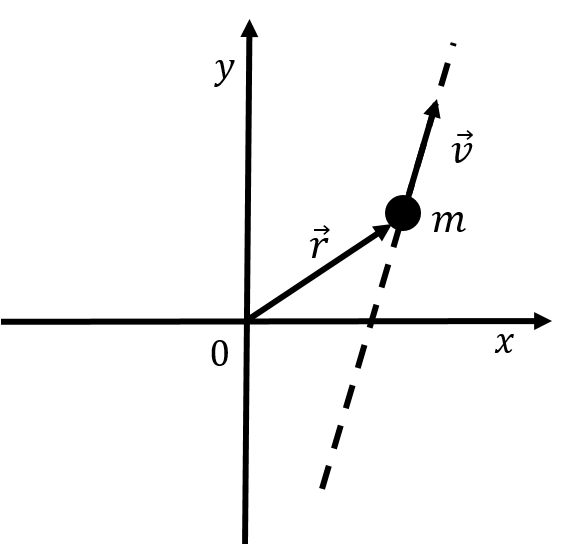
\includegraphics[width=0.3\linewidth]{files/line-7dfe9b02759d368dff3d32815c69cde0.png}
\caption[]{A particle moving in a straight line.}
\label{fig:angularmomentumrolling:line}
\end{figure}

A particle is moving with constant velocity $\vec v$ (in a straight line) relative to a coordinate system in an inertial frame of reference, as shown in Figure~\ref{fig:angularmomentumrolling:line}. Show that its angular momentum about the origin is conserved.

\begin{framed}
\textbf{Solution}\\
In this case, the particle is moving in a straight line, but we can still define its angular momentum relative to the origin. If $\vec r$ is the position vector of the particle relative to the origin, its angular momentum is:
\begin{equation}
\vec L = \vec r \times \vec p
\end{equation}
We can take the time derivative of the angular momentum to see if it changes with time:
\begin{equation}
\frac{d\vec L}{dt} = &= \frac{d}{dt} (\vec r\times \vec p)\\
&=\frac{d\vec r}{dt}\times \vec p + \vec r\times\frac{d\vec p}{dt}\\
&=\vec v\times \vec p + \vec r\times\frac{d\vec p}{dt}\\
\end{equation}
The first term is zero because $\vec v$ and $\vec p$ are parallel (so their cross-product must be zero). The second term is zero because the particle's momentum is constant in time (since its velocity is constant). Thus, the particle's angular momentum does not change with time, and it is conserved.

\textbf{Discussion:} Of course, we expected this result since no net torque is exerted on the particle. It is however worth highlighting that a particle does not need to be rotating for its angular momentum about a given axis to be defined or conserved; all that matters is that there is no net torque on the particle relative to that axis.
\end{framed}
\end{framed}

\paragraph{Angular momentum of an object or system}

Consider a system made of many particles of mass, $m_i$, each with a position, $\vec r_i$, and velocity, $\vec v_i$, relative to a point of rotation that is fixed in an inertial frame of reference.

We can write Newton's Second Law using the angular momentum, $\vec L_i$, for particle $i$:
\begin{equation}
\frac{d\vec L_i}{dt} = \vec \tau_i^{net}
\end{equation}
where $\vec \tau_i^{net}$ is the net torque exerted on particle $i$. We can sum each side of this equation for all of the particles in the system:
\begin{equation}
\frac{d\vec L_1}{dt} + \frac{d\vec L_2}{dt} + \frac{d\vec L_3}{dt} + \dots &= \vec \tau_1^{net} + \vec \tau_2^{net} +\vec \tau_3^{net} + \dots\\
\therefore \frac{d}{dt} \sum_i\vec L_i &= \sum_i \vec \tau_i^{net}
\end{equation}
The sum of all of the torques on all of the particles will include a sum over torques that are internal to the system and torques that are external to the system. The sum over internal torques is zero:
\begin{equation}
\sum_i \vec\tau_i^{net} = \sum_i \vec\tau_i^{int} + \sum_i \vec\tau_i^{ext} = \sum_i \vec\tau_i^{ext} = \vec\tau^{ext}
\end{equation}
where we defined, $\vec\tau^{ext}$, to be the net external torque exerted on the system. We also introduce the total angular momentum of the system, $\vec L$, as the sum of the angular momenta of the individual particles:
\begin{equation}
\vec L = \sum_i\vec L_i
\end{equation}
The rate of change of the total angular momentum of the system is then given by:
\begin{equation}
\boxed{\frac{d\vec L}{dt} = \vec \tau^{ext}}
\end{equation}

Up to this point, we did not require that the system be a solid object, so the particles in the system can move relative to each other. For example, the particles could be the Sun, planets, and everything else that is in our Solar System. The total angular momentum of all of the bodies in the Solar System (say, relative to the Sun) is conserved if there is no net torque on the solar system relative to the Sun (i.e. if there is no torque about the Sun exerted on any of the bodies in the system that is not exerted by one of the other bodies in the system).

Now, consider a solid object that is modelled as a system of many particles of mass, $m_i$, at position, $\vec r_i$, with velocity, $\vec v_i$, relative to a fixed axis of rotation. We can define the angular momentum of a single particle as equation (\ref{eq:angularmomentumrolling:liw}):
\begin{equation}
\vec L_i = m_i r_i^2 \vec \omega_i
\end{equation}
The total momentum of the system is the sum of the angular momenta of the individual particles:
\begin{equation}
\vec L &= \sum_i\vec L_i = \sum_i  m_i r_i^2 \vec \omega_i
\end{equation}
Because all of the particles are part of the same object, they must all move in unison and have the same angular velocity, $\vec\omega$, relative to the axis of rotation. We can thus define the angular momentum about the rotation axis for a solid object with angular velocity, $\vec\omega$, as:
\begin{equation}
\boxed{\vec L = \left(\sum_i  m_i r_i^2\right) \vec \omega = I\vec\omega}
\end{equation}
where we recognized that the sum in parentheses is simply the moment of inertia of the object relative to the axis of rotation. Again, it should be emphasized that this is the total angular momentum of the object about an axis of rotation, and not about a point.

Visualizing the torque and angular momentum of a system can be challenging because it almost always requires visualizing something in three dimensions. Consider a wheel (e.g. a bicycle wheel) that is spinning about horizontal axle which you hold with your hands, as illustrated in the left panel of Figure~\ref{fig:angularmomentumrolling:deltal} (without the hands). Imagine that you are holding onto the axle so that the wheel is front of you, your right hand is to the right of the wheel and your left hand is to the left of the wheel.

\begin{figure}[!htbp]
\centering
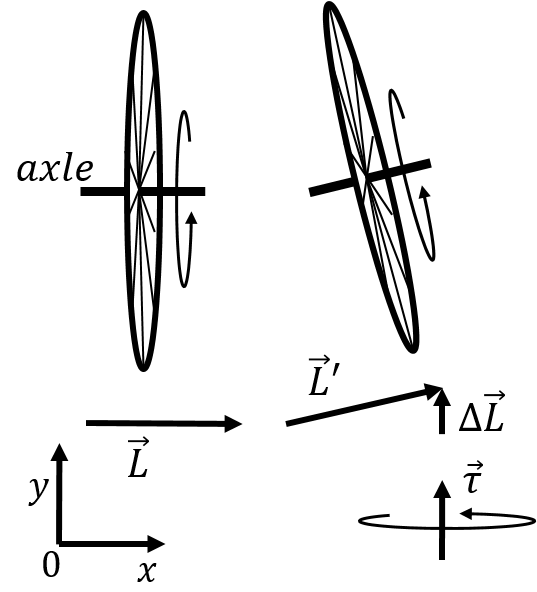
\includegraphics[width=0.4\linewidth]{files/deltal-b83960f835c131f13adeb1c0c670abe8.png}
\caption[]{A wheel rotating on an axle, with a horizontal angular velocity (left). If you try to tilt the axle as shown in the right panel, changing the angular momentum of the wheel, you will also need to exert a torque in the vertical direction (shown at the bottom right).}
\label{fig:angularmomentumrolling:deltal}
\end{figure}

We define a coordinate system as shown so that the wheel is spinning as shown in the left panel, with angular velocity (and angular momentum) in the positive $x$ direction (the top of the wheel is coming towards you).

You then try to lift your right hand while lowering your left hand in order to tilt the rotation axis, as shown in the right panel. In doing so, you change the direction of the angular momentum (and angular velocity) of the wheel such that the angular momentum, $\vec L'$, now has a vertical component, $\Delta \vec L$, as shown. The torque that is required in order to change the angular momentum is given by:
\begin{equation}
\vec \tau = \frac{d\vec L}{dt} \sim \frac{\Delta \vec L}{\Delta t}
\end{equation}
where $\Delta t$ is the time that it takes to change the axis of rotation. The torque required in order to change the axis of rotation is directed in the same direction as $\Delta \vec L$ (the positive $y$ direction). That is, you will not be able to simply tilt the axle as shown; if you want to tilt the axle, you will also need to push forward with you right hand and pull backwards with your left hand to exert the required torque (shown in the bottom right of the figure)! If you simply try to tilt the rotation axis, your right hand will be pushed towards you and your left hand away from you, as a reaction to the torque that would otherwise be required to tilt the axis!

\paragraph{Conservation of angular momentum}

In the previous section, we saw that the net external torque that is exerted on an object (or system) is equal to the rate of change of its angular momentum:
\begin{equation}
\frac{d\vec L}{dt} = \vec \tau^{ext}
\end{equation}
where the angular momentum and torque are measured about the same axis or point of rotation, fixed in an inertial frame of reference.

The total angular momentum of a system about a point of rotation is conserved (i.e. does not change with time) if there is no net external torque exerted on the system about that point. If one makes the system large enough, then all of the torques can be taken to be internal, and the angular momentum of the system is conserved. The angular momentum of the Universe about a fixed point is thus conserved.

Conservation of angular momentum is another conservation law that we derived from Newton's Second Law. In the modern formulation of physics, we understand that the conservation of angular momentum is associated with rotational symmetry of Newton's Second Law; it does not matter from which ``angle'' we model a system, we can always use Newton's Second Law. Similarly, conservation of linear momentum is associated with translational symmetry and conservation of energy is associated with the fact that Newton's Second Law does not change with time. Angular momentum is fundamentally different than linear momentum and energy, and is conserved under different conditions. The angular momentum of a system about a given axis/point is conserved if there is no net torque on the system about that axis/point.

\begin{framed}
\textbf{Example 11.5}\\
During a spin, a figure skater brings his arms close to his body and increases his angular velocity from $\omega_1$ to $\omega_2$. By what fraction did his moment of inertia decrease in doing so?

\begin{framed}
\textbf{Solution}\\
We can consider the rotation axis to be vertical through the centre of the skater. When the figure skater is spinning, there is no net external torque on him. Thus, his angular momentum is conserved as he bring his arms in. As he bring his arms in, his moment of inertia decreases, since he is bringing the mass of his arms closer to the axis of rotation. If $I_1$ and $I_2$ are the moments of inertia of the skater before and after brining his arms in, respectively, we can write the angular momentum about his axis of rotation as:
\begin{equation}
L_1 &= I_1\omega_1\\
L_2 &= I_2\omega_2
\end{equation}
Since there is no external torque on the skater, the angular momentum is the same before and after he changes his moment of inertia:
\begin{equation}
L_1 &= L_2\\
I_1\omega_1 &= I_2\omega_2\\
\therefore \frac{I_1}{I_2} &= \frac{\omega_2}{\omega_1}
\end{equation}
\textbf{Discussion:} A spinning figure skater is a good example of the conservation of angular momentum. By changing their shape, they can change their moment of inertia and thus their angular velocity.
\end{framed}
\end{framed}

\begin{framed}
\textbf{Example 11.6}\\
Show that Kepler's Second Law is equivalent to a statement about conservation of the angular momentum of a planet orbiting the Sun.

\begin{framed}
\textbf{Solution}\\
Kepler's Second Law states that in a period of time $\Delta t$, the area, $\Delta A$, that is swept out by a planet is constant, regardless of where it is along its orbit. In other words:
\begin{equation}
\frac{\Delta A}{\Delta t} = \text{constant}
\end{equation}
Figure~\ref{fig:angularmomentumrolling:kepler} shows a planet in an elliptical orbit around the sun.

\begin{figure}[!htbp]
\centering
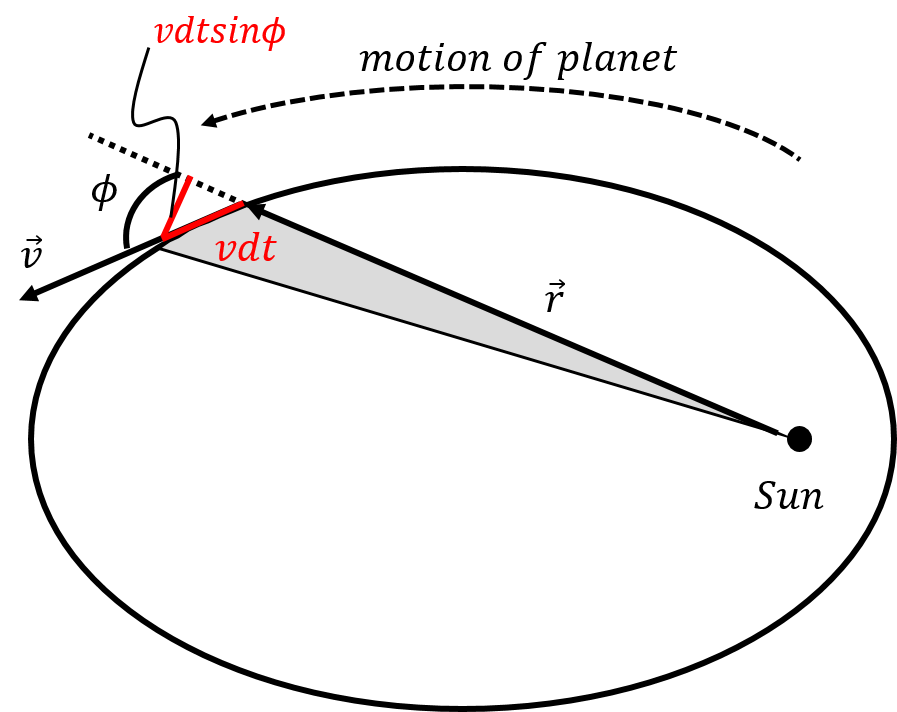
\includegraphics[width=0.5\linewidth]{files/kepler-4f0dc3c3a6aa1990dece4a276ade8e92.png}
\caption[]{The area swept out by a planet in a period of time $dt$.}
\label{fig:angularmomentumrolling:kepler}
\end{figure}

At some point in time, the planet has a velocity vector $\vec v$ and position vector $\vec r$ relative to the Sun. In a small period of time $dt$, the planet will move along a short distance $vdt$, which we can take as a straight line if $dt$ is small enough. Let $\phi$ be the angle between the velocity and position vectors when these are tail to tail, as illustrated.

The small amount of area, $dA$, swept out by the planet in a period of time $dt$, is given by the area of the right angle triangle with height $r$ and base $vdt\sin\phi$\footnote{This is only exact in the limit of $dt\to 0$, when the small area from the extra piece outside of the ellipse vanishes.}:
\begin{equation}
dA = \frac{1}{2} r vdt\sin\phi
\end{equation}
The rate at which the area is swept out is thus:
\begin{equation}
\frac{dA}{dt} =  \frac{1}{2} r v\sin\phi
\end{equation}
Consider now the magnitude of the planet's angular momentum about the Sun:
\begin{equation}
L = rp\sin\phi = rmv\sin\phi
\end{equation}
where the mass of the planet is $m$. The rate at which the planet sweeps out the area can be written in terms of the angular momentum of the planet:
\begin{equation}
\frac{dA}{dt} &=  \frac{1}{2} r v\sin\phi = \frac{L}{2m}
\end{equation}
The only force exerted on the planet is the gravitational force from the Sun. That force is always anti-parallel to the vector $\vec r$ from the Sun to the planet, and cannot result in a torque on the planet about the Sun. Thus, the angular momentum of the planet about the Sun must be conserved, and $L$ is constant. In turn, this means that the rate at which area is swept out by the planet, which is proportional to $L$, is also constant. Thus, Kepler's Second Law is equivalent to saying that the angular momentum of a planet relative to the Sun is constant.
\end{framed}
\end{framed}

\subsubsection{Summary}

If an object is rotating with angular speed, $\omega$, about an axis that is fixed in an inertial frame of reference, the rotational kinetic energy of that object is given by:
\begin{equation}
K_{rot} = \frac{1}{2}I\omega^2
\end{equation}
where $I$ is the moment of inertia of that object about the axis of rotation.

The net work done by the net torque exerted on an object about a fixed axis or rotation in an inertial frame of reference is equal to object's change in rotational kinetic energy:
\begin{equation}
W = \int_{\theta_1}^{\theta_2}\vec \tau^{net}\cdot d\vec \theta = \frac{1}{2}I\omega_2^2 -\frac{1}{2}I\omega_1^2
\end{equation}
If a torque, $\vec \tau$, about a stationary axis is exerted on an object that is rotating with a constant angular velocity, $\vec \omega$, about that axis, then the torque does work at a rate:
\begin{equation}
P = \vec \tau \cdot \vec \omega
\end{equation}

If an object of mass, $M$, is rotating about an axis through its centre of mass, and the centre of mass of is moving with speed, $v_{CM}$, relative to an inertial frame of reference, then the total kinetic energy of the object is given by:
\begin{equation}
K_{tot} = K_{rot} + K_{trans} = \frac{1}{2}I_{CM}\omega^2+ \frac{1}{2}Mv_{CM}^2
\end{equation}
where, $\omega$, is the angular speed of the object about the centre of mass, and, $I_{CM}$, is the moment of inertia of the object about the centre of mass. The two terms in the kinetic energy come from the rotation about the centre of mass ($K_{rot}$), and the translational motion of the centre of mass ($K_{trans}$).

An object is said to be rolling without slipping on a surface if the point on the object that is in contact with the surface is instantaneously at rest relative to the surface. We can model an object that is rolling without slipping by superimposing rotational motion about the centre of mass with translational motion of the centre of mass. The angular speed, $\omega$, and the angular acceleration, $\alpha$, of the object about an axis through its centre of mass are related to the speed, $v_{CM}$, and linear acceleration, $a_{CM}$, of the centre of mass, respectively:
\begin{equation}
v_{CM} &= \omega R\\
a_{CM} &= \alpha R
\end{equation}
These conditions are equivalent to stating that the object is rolling without slipping.

When an object is rolling without slipping, we can also model its motion as if it were instantaneously rotating about an axis that goes through the point of contact between the object and the ground (the instantaneous axis of rotation). The angular speed (and acceleration) about the instantaneous axis of rotation are the same as they are when the object is modelled as rotating about its (moving) centre of mass.

An object can only be rolling without slipping if there is a force of static friction exerted by the surface on the object. Without this force, the object would slip along the surface.

We can define the angular momentum of a particle, $\vec L$, about a point in an inertial frame of reference as:
\begin{equation}
\vec L = \vec r \times \vec p
\end{equation}
where, $\vec r$, is the vector from the point to the particle, and, $\vec p$, is the linear momentum of the particle. If the particle has an angular velocity, $\vec\omega$, relative to an axis of rotation its angular momentum about that axis can be written as:
\begin{equation}
\vec L = mr^2\vec\omega = I\vec\omega
\end{equation}
where, $r$, is the distance between the particle and the axis of rotation, and $I=mr^2$, can be thought of as the moment of inertia of the particle about that axis.

We can write the equivalent of Newton's Second Law for the rotational dynamics of a particle using angular momentum:
\begin{equation}
\frac{d\vec L}{dt}=\vec\tau^{net}
\end{equation}
where, $\vec \tau^{net}$, is the net torque on the particle about the same point used to define angular momentum. That point must be in an inertial frame of reference.

The rate of change of the total angular momentum for a system of particles, $\vec L=\vec L_1 + \vec L_2 +\dots$, about a given point is given by:
\begin{equation}
\frac{d\vec L}{dt}=\vec\tau^{ext}
\end{equation}
where, $\vec\tau^{ext}$, is the net external torque on the system about the point of rotation. If the net external torque of the system is zero, then the total angular momentum of the system is constant (conserved). Again, the point of rotation must be in an inertial frame of reference\footnote{Technically, if the point is the centre of mass, then this is valid even in an accelerating frame of reference.}.

For a solid object, in which all of the particles must move in unison, we can define the angular momentum of the object about a stationary axis to be:
\begin{equation}
\vec L = I\vec \omega
\end{equation}
where, $\vec\omega$, is the angular velocity of the object about that axis, and, $I$, is the object's corresponding moment of inertia about that axis.

Many of the relations that exist between linear quantities have an analogue relation between the corresponding angular quantities, as summarized in the table below:

\begin{table}
\centering
\begin{tabular}{p{\dimexpr 0.250\linewidth-2\tabcolsep}p{\dimexpr 0.250\linewidth-2\tabcolsep}p{\dimexpr 0.250\linewidth-2\tabcolsep}p{\dimexpr 0.250\linewidth-2\tabcolsep}}
\toprule
\textbf{Name} & \textbf{Linear} & \textbf{Angular} & \textbf{Correspondence} \\
\hline
Displacement & $s$ & $\vec \theta$ & $d\vec\theta=\frac{1}{r^2} \vec r\times d\vec s$ \\
Velocity & $\vec v$ & $\vec \omega$ & $\vec\omega=\frac{1}{r^2} \vec r\times \vec v$, $v_s = \vec\omega\times \vec r$\footnote{This corresponds to the component of velocity perpendicular to $\vec r$.} \\
Acceleration & $\vec a$ & $\vec \alpha$ & $\vec\alpha=\frac{1}{r^2} \vec r\times \vec a$, $a_s = \vec\alpha\times \vec r$\footnote{This corresponds to the component of acceleration perpendicular to $\vec r$.\}} \\
Inertia & $m$ & $I$ & $I=\sum_i m_ir_i^2$ \\
Momentum & $\vec p=m\vec v$ & $\vec L = I\vec \omega$ & $\vec L = \vec r\times \vec p$ \\
Newton's Second Law & $\vec F^{ext}=m\vec a_{CM}$ & $\vec \tau^{ext} = I\vec\alpha$ & $\vec F \to \vec\tau$, $m\to I$, $\vec a \to \vec \alpha$ \\
Newton's Second Law & $\frac{d\vec p}{dt} =\vec F^{ext}$ & $\frac{d\vec L}{dt} =\vec \tau^{ext}$ & $\vec F \to \vec\tau$, $\vec p \to \vec L$ \\
Kinetic energy & $\frac{1}{2}mv^2$ & $\frac{1}{2}I\omega^2$ & $m\to I$, $v\to \omega$ \\
Power & $\vec F \cdot \vec v$ & $\vec \tau \cdot \vec\omega$ & $\vec F \to \vec\tau$, $\vec v\to \vec\omega$ \\
\bottomrule
\end{tabular}
\end{table}

\begin{framed}
\textbf{Important Equations}\\
\textbf{Rotational kinetic energy of a rotating object:}
\begin{equation}
K_{rot} = \frac{1}{2}I\omega^2
\end{equation}
\textbf{Total kinetic energy:}
\begin{equation}
K_{tot} = K_{rot} + K_{trans} = \frac{1}{2}I_{CM}\omega^2+ \frac{1}{2}Mv_{CM}^2
\end{equation}
\textbf{Work:}
\begin{equation}
W = \int_{\theta_1}^{\theta_2}\vec \tau^{net}\cdot d\vec \theta = \frac{1}{2}I\omega_2^2 -\frac{1}{2}I\omega_1^2
\end{equation}
\textbf{Power:}
\begin{equation}
P = \vec \tau \cdot \vec \omega
\end{equation}

\textbf{Angular momentum:}
\begin{equation}
\vec L = \vec r \times \vec p\\
\vec L = mr^2\vec\omega = I\vec\omega\\
\frac{d\vec L}{dt}=\vec\tau^{net}\\
\frac{d\vec L}{dt}=\vec\tau^{ext}\\
\vec L = I\vec \omega\\
\end{equation}
\end{framed}

\begin{framed}
\textbf{Important Definitions}\\
\begin{itemize}
\item \textbf{Angular momentum:} The rotational equivalent of linear momentum. Angular momentum must be defined relative to an axis of rotation. SI units: ${\rm \left[{kg\cdot m^2\cdot s^{ -1}}\right]}$. Common variable(s): $\vec L$.
\item \textbf{Rotational kinetic energy:} The rotational equivalent of translation kinetic energy. Generally, an object can have both rotational and translational kinetic energy.  SI units: ${\rm \left[{J}\right]}$. Common variables: $K_{rot}$.
\end{itemize}
\end{framed}

\subsubsection{Thinking about the material}

\begin{framed}
\textbf{Reflect and research}\\
\begin{itemize}
\item How can a bicycle move forward? Draw the external forces on the bicycle that are required for the wheels to turn.
\item Does conservation of angular momentum play a role in being able to remain upright on a bicyle? If yes, how?
\item How does an anti-lock braking system (ABS) provide better breaking for your car? What is the physics behind this?
\end{itemize}
\end{framed}

\begin{framed}
\textbf{To try at home}\\
\begin{itemize}
\item Describe how you can qualitatively confirm conservation of angular momentum.
\end{itemize}
\end{framed}

\begin{framed}
\textbf{To try in the lab}\\
\begin{itemize}
\item Propose an experiment to measure the critical angle of an incline, above which a given object cannot roll without slipping, and compare this to a model prediction.
\item Propose an experiment to test the conservation of angular momentum of a rotating object.
\item Propose an experiment to test whether an object with constant velocity can impart angular momentum to another object.
\end{itemize}
\end{framed}

\subsubsection{Sample problems and solutions}

\paragraph{Problems}

\begin{framed}
\textbf{Problem}\\
A yo-yo can be modelled as two uniform disks, of radius $R_2$, attached to either side of a smaller uniform disk of radius $R_1$, as in Figure~\ref{fig:angularmomentumrolling:yoyo}. We can assume that all three disks have a mass $m$. A mass-less string is wrapped around the smaller disk and then the yo-yo is released. What is the acceleration of the centre of mass of the yo-yo as it falls and the string unwinds?

\begin{figure}[!htbp]
\centering
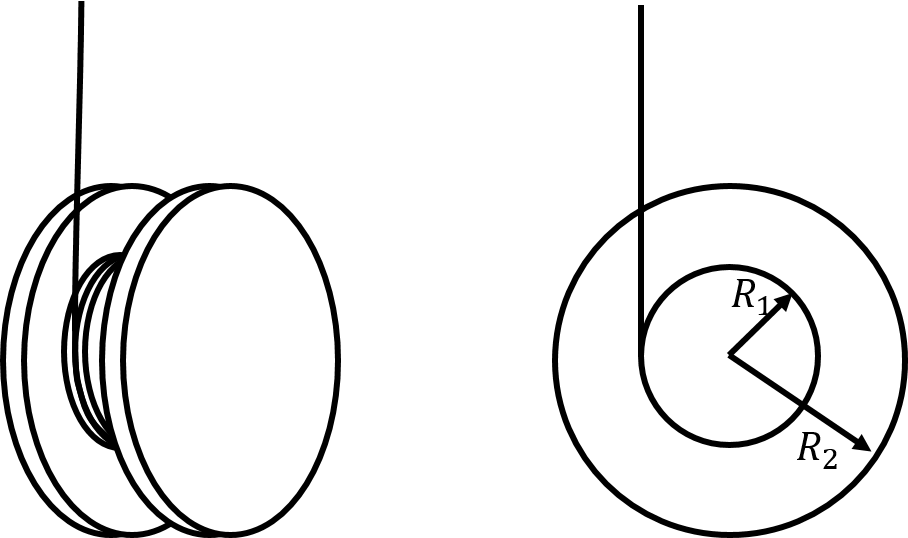
\includegraphics[width=0.5\linewidth]{files/yoyo-8fcc3b35b0626567c8d6c678f4922917.png}
\caption[]{Left: Side view of the yo-yo. Right: Front view of the yo-yo, modelled as two disks of radius of $R_2$ attached to either side of a disk of radius $R_1$.}
\label{fig:angularmomentumrolling:yoyo}
\end{figure}
\end{framed}

\begin{framed}
\textbf{Problem}\\
\begin{figure}[!htbp]
\centering
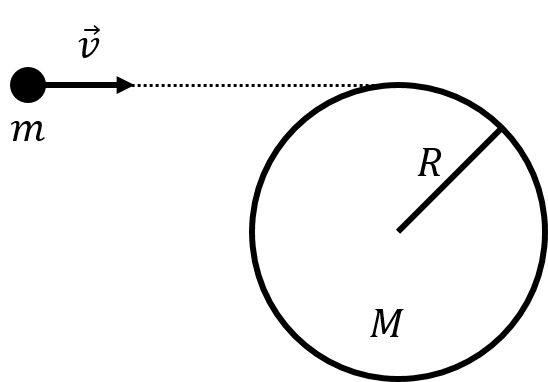
\includegraphics[width=0.3\linewidth]{files/balldisk-68702f5e17e23a584057698b0fa628f4.png}
\caption[]{A projectile of mass $m$ is about to collide with a disk that can spin about its axis of symmetry. View from above.}
\label{fig:angularmomentumrolling:balldisk}
\end{figure}

A projectile of mass $m$ is fired towards a stationary disk of radius $R$ and mass $M$ that lies on a horizontal table, as depicted from above in Figure~\ref{fig:angularmomentumrolling:balldisk}. The disk is in the horizontal plane and can rotate about a vertical axis through its centre. The axle about which the disk rotates is attached to the table and cannot move. The projectile's velocity, $\vec v$, is horizontal and such that the projectile embeds itself at the edge of the disk.  What is the angular velocity of the disk, about its centre, after the projectile has embedded itself into the disk? Was the collision elastic? Was linear momentum conserved during the collision?
\end{framed}

\paragraph{Solutions}

\begin{framed}
\textbf{Solution}\\
The forces acting on the yo-yo are:

\begin{itemize}
\item $\vec F_g$, its weight, with magnitude $3mg$.
\item $\vec T$, a force of tension from the string.
\end{itemize}

The forces, where they are exerted, and our choice of coordinate system are shown in Figure~\ref{fig:angularmomentumrolling:yoyo_fbd}.

\begin{figure}[!htbp]
\centering
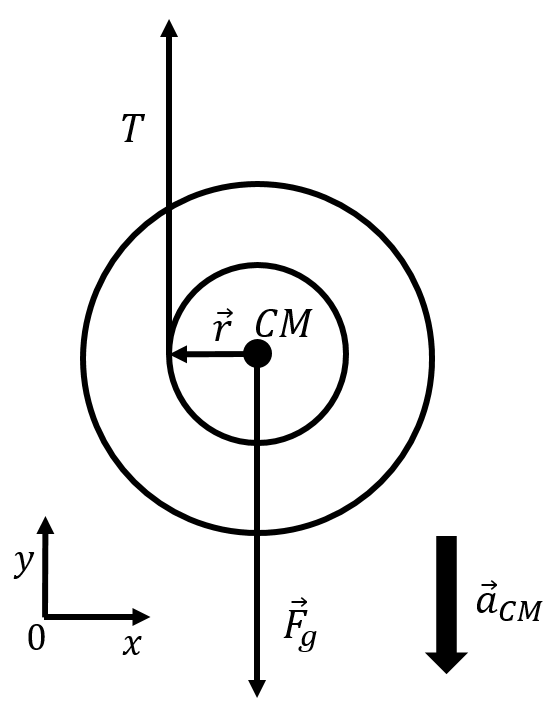
\includegraphics[width=0.3\linewidth]{files/yoyo_fbd-ecc661c3724d09f92dbaf7fbbadd684d.png}
\caption[]{Free body diagram for the yo-yo.}
\label{fig:angularmomentumrolling:yoyo_fbd}
\end{figure}

The yo-yo can be modelled as rolling without slipping, as if it were rolling along the string that unwinds. The torque about the centre of mass is provided by the tension in the string. The angular acceleration of the yo-yo, $\alpha$, will be related to the linear acceleration of the centre of mass, $\vec a_{CM}$, since this is rolling without slipping:
\begin{equation}
a_{CM}=\alpha R_1
\end{equation}
where $R_1$ is the radius that is analogous to rolling motion. Since the torque from the force of gravity is zero, we can write Newton's Second Law for rotational quantities as:
\begin{equation}
\vec\tau^{ext}&=I\vec\alpha\\
TR_1 &= I\alpha
\end{equation}
where $TR_1$ is the magnitude of the torque from the force of tension, since the tension is perpendicular to the vector $\vec r$ between the centre of mass and the point where the tension is exerted. The moment of inertia of the yo-yo about its centre of mass is the sum of the moments of inertia of the three disks about their axis of symmetry:
\begin{equation}
I=\frac{1}{2}MR_2^2 +\frac{1}{2} MR_2^2+\frac{1}{2}MR_1^2=\frac{1}{2}M(2R_2^2+R_1^2)
\end{equation}
We can also write Newton's Second Law in the vertical direction for the yo-yo (of mass $3M$):
\begin{equation}
\sum F_y = -F_g + T &= -3Ma_{CM}\\
-3Mg + T = -3Ma_{CM}
\end{equation}
where we $a_{CM}$ is the magnitude of the acceleration of the centre of mass (since we included the sign in the first equation).

We can eliminate the unknown force of tension from the equations by substitution. Using the equation from Newton's Second Law:
\begin{equation}
T=3M (g-a_{CM})
\end{equation}
and substituting this into the rotational equation:
\begin{equation}
TR_1 &= I\alpha\\
3M (g-a_{CM}) R_1 &=  I\alpha
\end{equation}
We can solve for $a_{CM}$ by using the condition for rolling without slipping ($\alpha R_1 = a_{CM}$):
\begin{equation}
3M (g-a_{CM}) R_1 &=  I\frac{a_{CM}}{R_1}\\
\frac{I}{R_1}a_{CM}+3MR_1a_{CM}&= 3MgR_1\\
a_{CM}\left(\frac{I}{R_1}+3MR_1\right)&= 3MgR_1\\
a_{CM}&=\frac{3MgR_1}{\frac{I}{R_1}+3MR_1}\\
&=\frac{3MgR_1}{\frac{\frac{1}{2}M(2R_2^2+R_1^2)}{R_1}+3MR_1}\\
&=\left(\frac{3R_1^2}{\frac{1}{2}(2R_2^2+R_1^2)+3R_1^2}\right)g\\
\therefore a_{CM}&=\left( \frac{3R_1^2}{R_2^2+\frac{7}{2}R_1^2}\right)g
\end{equation}
\end{framed}

\begin{framed}
\textbf{Solution}\\
We consider the projectile and disk as a system, and a rotation axis that passes through the centre of disk. There are no external torques exerted on the system about the rotation axis, so the angular momentum of the system must be conserved through the collision. Before the collision, only the projectile has angular momentum about the axis of rotation, so the magnitude of the angular momentum before the collision is:
\begin{equation}
L = rp\sin\phi
\end{equation}
where $\phi$ is the angle between the particle's momentum, $\vec p=m\vec v$, and a vector, $\vec r$, from the axis of rotation to the particle. We can calculate the particle's angular momentum just before the collision, so that $\vec r$ is the vector from the centre of the circle to the point where the particle collides (with magnitude $R$, and perpendicular to $\vec v$). The initial angular momentum of the system is thus:
\begin{equation}
L=rp=Rmv
\end{equation}
After the collision, the projectile is embedded in the disk. The resulting object has a moment of inertia given by:
\begin{equation}
I = I_{disk}+ I_{particle} = \frac{1}{2}MR^2+mR^2
\end{equation}
After the collision, the angular momentum of the disk with the embedded projectile is given by:
\begin{equation}
L'=I\omega = \left(\frac{1}{2}M+m\right)R^2\omega
\end{equation}
Using conservation of angular momentum, the angular velocity of the disk after the collision is:
\begin{equation}
L &= L'\\
Rmv &= \left(\frac{1}{2}M+m\right)R^2\omega\\
\therefore \omega &= \frac{mv}{\left(\frac{1}{2}M+m\right)R}
\end{equation}
We do not expect that mechanical energy is conserved during the collision, since the projectile embeds itself, which must cost energy. The mechanical energy before the collision is given by the kinetic energy of the projectile:
\begin{equation}
E = \frac{1}{2}mv^2
\end{equation}
After the collision, the kinetic energy is the rotational kinetic energy of the disk with embedded projectile about the axis of rotation:
\begin{equation}
E' &= \frac{1}{2}I\omega^2 = \frac{1}{2} \left(\frac{1}{2}M+m\right)R^2 \left( \frac{mv}{\left(\frac{1}{2}M+m\right)R}\right)^2\\
&= \frac{1}{2} \frac{m^2}{\left(\frac{1}{2}M+m\right)} v^2
\end{equation}
We can see that $E'$ is less than $E$, by taking their ratio:
\begin{equation}
\frac{E'}{E} &= \frac{\frac{1}{2} \frac{m^2}{\left(\frac{1}{2}M+m\right)} v^2}{\frac{1}{2}mv^2}\\
&=\frac{m}{\left(\frac{1}{2}M+m\right)}<1
\end{equation}
and we confirm that mechanical energy is not conserved in the collision (and that energy was lost since one had to deform the projectile and disk).

Linear momentum is clearly not conserved since the final linear momentum is zero, whereas before the collision, it is $\vec p=m\vec v$. The centre of mass of the disk+projectile system moves before the collision and not after. There must thus be a net external force that is exerted on the system. That force is exerted by the table onto the axle of disk, as the disk would otherwise recoil when hit with the projectile.

\textbf{Discussion:} In this example, we used conservation of angular momentum to model a collision. The collision is inelastic, because the projectile embeds itself into the disk. The linear momentum is not conserved through the collision because the axle about which the disk rotates must exert a force on the disk to prevent it from recoiling.
\end{framed}